\chap{Thymio est sur un piste}\label{ch.line}

Imaginez un entrepôt gigantesque. Des robots sont désignés pour aller chercher ou déposer du matériel à l'intérieur. Il leur faut un moyen de retrouver leur chemin. Nous pourrions peindre des lignes sur le sol pour les guider!

\begin{bclogo}[couleur = pink!30, arrondi = 0.1, logo = \bccrayon, ombre = true]{Challenge!}Écrivez un programme en utilisant VPL qui permet à Thymio de suivre une ligne noir sur une table blanche!
\end{bclogo}

{\raggedleft \hfill Programme \bu{follow-line.aesl}}

Suivre une ligne sur le sol est un bon exemple du genre de difficultés rencontrées en robotique. La ligne peut-être mal dessinée, de la poussière ou de la saleté peut la recouvrir, le robot peut rencontrer des obstacles... Il faut donc créer, ce que nous appelons,  un contrôleur. Il aura pour tâche de dicter la vitesse du robot, sa direction, etc...

\sect{Quel genre de ligne}

Pour suivre une ligne, nous allons utiliser les détecteurs de sol que nous avons déjà utilisé dans \cref{Chap.Thymio.bouge}. Rappelons qu'il s'agit des même capteurs que ceux qui se trouve à l'avant et à l'arrière de Thymio. Ils envoient de la lumière infrarouge (invisible pour l'oeil humain) et regarde combien de cette lumière est renvoyée.

Si vous poser Thymio sur une table blanche, ou du moins de couleur claire, beaucoup de lumière sera réfléchie, donc cet événement sera déclenché: \blk{lots-of-light}. Au contraire, si Thymio se trouve sur une surface foncée, noir par exemple, seulement un peu de lumière sera réfléchie, c'est donc cet événement-ci qui sera déclenché: \blk{little-light}.

Pour détecter une ligne, Thymio doit donc suivre une trace sombre sur un environnement claire, ou l'inverse. Vous pouvez donc dessiner ou peindre une ligne noire sur une feuille blanche. Vous pouvez également utiliser un gros scotch noir que vous coller sur une table blanche, par exemple. La ligne devrait faire au minimum 5 centimètres de large pour que les deux capteurs sous Thymio puisse la détecter. Vous pouvez voir un exemple sur \cref{fig.tape}.

\begin{figure}
\begin{center}
\gr{blacktape}{.5}
\caption{Thymio suit une ligne de scotch noir}\label{fig.tape}
\end{center}
\end{figure}


\begin{bclogo}[couleur = blue!30, arrondi = 0.1, logo = \bcinfo, ombre = true]{Truc et astuce!}Pour profiter pleinement de Thymio, assurez-vous d'avoir un câble USB assez long, des rallonges peuvent être trouvées dans tous les magasins d'informatique.
\end{bclogo}

\sect{Thymio s'arrête, Thymio avance}

Le premier pas pour faire suivre une ligne à Thymio est de le faire avancer s'il est sur la ligne et de le faire s'arrêter s'il ne se trouve pas sur cette dernière. Comme expliqué précédemment, si Thymio se trouve sur une surface blanche, donc à côté de la ligne, beaucoup de lumière sera réfléchie sur ses capteurs inférieurs. Il faut donc qu'il s'arrête puisqu'il n'est pas sur la ligne. Ensuite, si Thymio se trouve sur la ligne, peu de lumière sera réfléchie sur ses capteurs inférieurs. Il faut donc le faire avancer s'il ne détecte que peu de lumière. Nous avons donc deux paires événement-action qui sont illustrée sur \cref{fig.start-stop}.

\begin{figure}[h]
\begin{center}
\gr{line-forward}{.3}
\caption{Thymio s'arrête, Thymio avance}\label{fig.start-stop}
\end{center}
\end{figure}

\sect{Votre premier contrôleur}

Maintenant, il s'agit de créer un contrôleur qui va faire suivre la ligne à Thymio. Le programme que vous avez fait jusqu'à maintenant fera s'arrêter Thymio dès qu'un de ses deux capteurs inférieurs verra qu'il n'est plus sur la ligne. Pour le faire suivre la ligne plutôt que s'arrêter dès qu'un des capteurs la quitte, il faut que: 

\begin{itemize}
	\item si Thymio se trouve à moitié sur la ligne, un peu trop à droite, il tourne à gauche afin de se remettre sur la ligne, comme illustré sur \cref{fig.too-right}.
	\item  si Thymio se trouve à moitié sur la ligne, un peu trop à gauche, il tourne à droite afin de se remettre sur la ligne.
\end{itemize}

Comme nous avons deux conditions, il nous faut deux paires événement-action, comme illustré sur\cref{fig.follow-line}.

\begin{figure}[h]
    \centering
    \subfigure[Thymio à moitié sur la ligne, vue du dessus]{ \label{fig.too-right} \includegraphics[width = 0.3\textwidth]{thymio_ligne}}
    \hspace{1cm}
    \subfigure[Trop à droite\ldots Trop à gauche]{ \label{fig.follow-line} 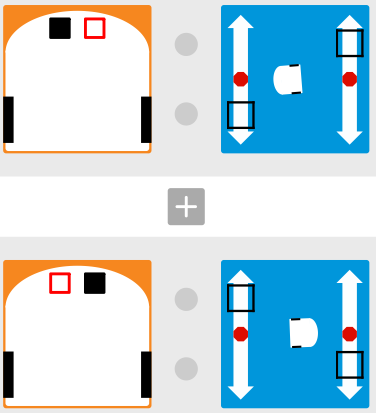
\includegraphics[width = 0.36\textwidth]{line-controller}}
    \caption{Un contrôleur pour suivre une ligne}
\end{figure}

\sect{Régler les paramètres}

Il est assez facile de comprendre que Thymio doit tourner à gauche s'il est trop à droite de la ligne et vis-versa. La vraie question est plutôt de combien doit-il tourner? Doit-il s'arrêter et tourner sur lui-même? Doit-il simplement corriger légèrement? Ou au contraire de manière plus sèche? C'est tout l'art de la création de contrôleur que de \textit{régler les paramètres} de ce contrôleur.

Mais qu'est que sont ces \textit{paramètres}?

Ils varient totalement d'une application à une autre. Ils sont des entités que le créateur du contrôleur doit choisir afin d'obtenir le comportement désiré. Dans notre cas, il s'agit de la vitesses des roues dans les différents cas possibles. 

Thymio doit-il aller vite lorsqu'il est sur la ligne ou, au contraire, lentement? En allant vite, vous améliorerez son efficacité pour se déplacer d'un point à un autre mais vous risquez de le faire quitter la ligne avant qu'il ne se rende compte qu'il est en train de sortir, un peu comme si vous allez trop vite en voiture dans un virage serré. Pour ce \textit{paramètre}, il faudra trouver un bon compromis.

Une fois que Thymio remarque qu'il quitte la ligne, que doit-il faire? S'il s'arrête complètement et tourne sur lui-même, vous vous assurez qu'il ne quitte pas la ligne mais ses mouvements seront très saccadés. S'il corrige simplement sa trajectoire en diminuant la vitesse d'une roue, il se déplacera avec fluidité, mais il risque de quitter complètement la ligne\ldots 

Là aussi, il faudra trouver un bon compromis.

\begin{bclogo}[couleur = pink!30, arrondi = 0.1, logo = \bccrayon, ombre = true]{Challenge!}Thymio s'arrête complètement s'il ne détecte plus du tout la ligne. Modifiez le programme pour qu'il tourne lentement sur lui même s'il ne détecte plus du tout la ligne. Arrive-t-il à retrouver la ligne s'il la perd complètement? Essayer d'augmenter de plus en plus la vitesse des roues lorsqu'il est sur la ligne. Arrive-t-il à gérer un virage serré?
\end{bclogo}


\begin{bclogo}[couleur = pink!30, arrondi = 0.1, logo = \bccrayon, ombre = true]{Challenge!}Jouez avec la forme du parcours:

\begin{itemize}
\item Virages serrés
\item Virages doux
\item Zig-zag
\item Ligne plus large
\item Ligne plus étroite
\end{itemize}

Faites la course avec vos amis et votre famille. Qui arrive à faire le contrôleur le plus efficace? Y a-t-il un contrôleur parfait ou doit-il dépendre du parcours?
\end{bclogo}
